\section{Eksperymety}
\label{sec:exp}
\subsection{Testowe dane oraz zapytania}
\paragraph{Testowe dane}
Przeprowadziliśmy testy wydajności czasu konstrukcji jak i czasu zapytań wszystkich zaimplementowanych algorytmów i struktur danych. W celu przeprowadzenia testów wygenerowaliśmy przykładowe tablice o rozmiarze w przedziale od $1000$ do $4000000$ elementów. Tablice te podzieliliśmy na trzy kategorie w zależności od liczby unikalnych elementów: $\dt = 64, \dt=\sqrt{n}$ oraz $\dt = n/64$.
\paragraph{Testowe zapytania} Dla każdej tablicy o rozmiarze $n$ wygenerowaliśmy $n$ zapytań. Ponadto, każde zapytanie reprezentowaliśmy jako wylosowanie jednostajnie dwie liczby $i, j \in \{1,2,\dots,n\}$, które odpowiadają zapytaniu o przedział $A[\min(i, j) : \max(i, j)]$. Przez takie dobranie zapytań do danych, każde zapytanie ma oczekiwaną długość $1/3n$. Długość przedziału ma szczególne znaczenie dla algorytmów naiwnych, których to czas zapytania jest bezpośrednio od niej uzależniony. Ponadto, dla algorytmów offline wygenerowaliśmy dodatkowe testy ze zmienną liczbą zapytań, aby zbadać jaki faktyczny ma to wpływ na czas zapytania.
\begin{table}[]
    \centering
    \begin{tabular}{|l|l|}
        \hline
      \multicolumn{2}{|c|}{\textbf{Oprogramowanie}} \tabularnewline
      \hline 
      System operacyjny & Ubuntu 20.04 LTS \tabularnewline
      \hline 
     Wersja jądra & 5.4\tabularnewline
      \hline
      \multicolumn{2}{|c|}{\textbf{Sprzęt}} \tabularnewline
      \hline 
      Procesor & Intel Xeon Gold 6154 CPU @ 3.00GHz\tabularnewline
      \hline
     Pamięć podręczna L1/L2/L3 & 32KiB/1MiB/24MiB\tabularnewline
      \hline
      Drożność pamięci podręcznej & 8\tabularnewline
      \hline
      \hline
      Użyte rozszerzenia procesora & AVX512VL, MBI2 \tabularnewline
      \hline
    \end{tabular}
    \caption{Sprzęt oraz jego oprogramowanie na którym zostały przeprowadzone eksperymenty}
    \label{tab:my_label}
\end{table}

\subsection{Algorytm naiwny}
\subsubsection{Czas inicjalizacji}
\begin{minipage}[t]{0.5\textwidth}
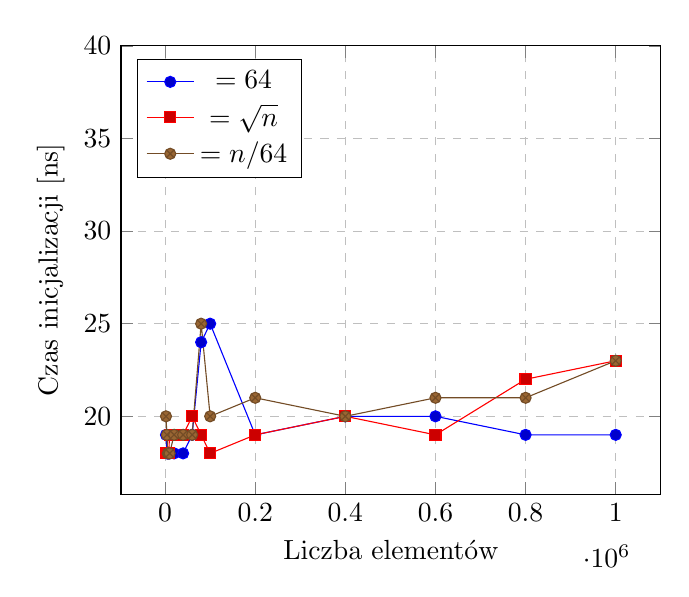
\begin{tikzpicture}
\begin{axis}[
    xlabel={Liczba elementów},
    ylabel={Czas inicjalizacji [ns]},
    ymax=40,
    ytick={20, 25, 30, 35, 40},
    xmajorgrids=true,
    ymajorgrids=true,
    grid style=dashed,
    legend pos=north west,
]
\addplot coordinates{(2000, 19)(4000, 18)(6000, 18)(8000, 18)(10000, 18)(20000, 18)(40000, 18)(60000, 19)(80000, 24)(100000, 25)(200000, 19)(400000, 20)(600000, 20)(800000, 19)(1000000, 19)};
\addplot coordinates{(2000, 18)(4000, 18)(6000, 18)(8000, 18)(10000, 19)(20000, 19)(40000, 19)(60000, 20)(80000, 19)(100000, 18)(200000, 19)(400000, 20)(600000, 19)(800000, 22)(1000000, 23)};
\addplot coordinates{(2000, 20)(4000, 19)(6000, 18)(8000, 18)(10000, 18)(20000, 19)(40000, 19)(60000, 19)(80000, 25)(100000, 20)(200000, 21)(400000, 20)(600000, 21)(800000, 21)(1000000, 23)};
\legend{$\dt=64$,$\dt=\sqrt{n}$,$\dt={n/64}$}
\end{axis}
\end{tikzpicture}
\captionof{figure}{Czas inicjalizacji algorytmu naiwnego}
\label{fig:plot-init-naive}
\end{minipage}
\hfill
\begin{minipage}[t]{0.49\textwidth}
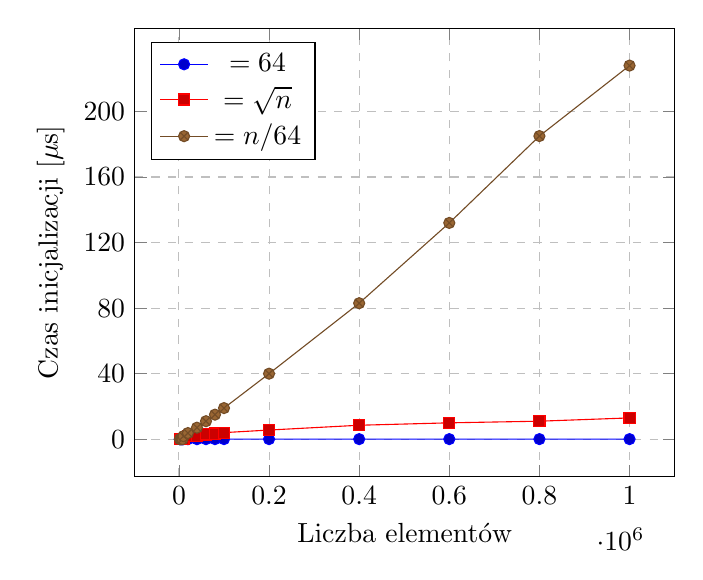
\begin{tikzpicture}
\begin{axis}[
    xlabel={Liczba elementów},
    ylabel={Czas inicjalizacji [$\mu$s]},
    ytick={0, 40, 80, 120, 160, 200},
    xmajorgrids=true,
    ymajorgrids=true,
    grid style=dashed,
    % xmode=log,
    % ymode=log,
    legend pos=north west,
]
\addplot coordinates{(2000, 0.031)(4000, 0.032)(6000, 0.030)(8000, 0.029)(10000, 0.029)(20000, 0.029)(40000, 0.030)(60000, 0.049)(80000, 0.063)(100000, 0.068)(200000, 0.059)(400000, 0.058)(600000, 0.058)(800000, 0.070)(1000000, 0.059)};
\addplot coordinates{(2000, 0.030)(4000, 0.034)(6000, 0.030)(8000, 0.032)(10000, 0.035)(20000, 1.749)(40000, 2.181)(60000, 2.932)(80000, 3.481)(100000, 4.033)(200000, 5.605)(400000, 8.528)(600000, 10)(800000, 11)(1000000, 13)};
\addplot coordinates{(2000, 0.028)(4000, 0.029)(6000, 0.033)(8000, 0.033)(10000, 1.894)(20000, 3.767)(40000, 7.055)(60000, 11)(80000, 15)(100000, 19)(200000, 40)(400000, 83)(600000, 132)(800000, 185)(1000000, 228)};
\legend{$\dt=64$,$\dt=\sqrt{n}$,$\dt={n/64}$}
\end{axis}
\end{tikzpicture}
\captionof{figure}{Czas inicjalizacji algorytmu naiwnego wariantu drugiego}
\label{fig:plot-init-naive-variants}
\end{minipage}
Czas inicjalizacji wariantu pierwszego jest praktycznie zerowy, w naszej implementacji zapamiętujemy wskaźnik do tablicy na której będziemy wykonywać zapytania. Z drugiej strony podczas inicjalizacji wariantu drugiego tworzymy tablicę zastępującą hash-mapie w wariancie pierwszym. Moglibyśmy ją tworzyć za każdym razem podczas zapytania, aczkolwiek czas zapytania wzrósłby z $\Oh(j-i)$ do $\Oh(max(\dt, j-i))$. Jak widać na rysunku \ref{fig:plot-init-naive-variants}, czas inicjalizacji rośnie wraz z $\dt$, aczkolwiek pomijalnie mało w porównaniu do czasu pojedynczego zapytania.\vspace{-0.5em}
\subsubsection{Czas zapytania}
\begin{minipage}[t]{0.5\textwidth}
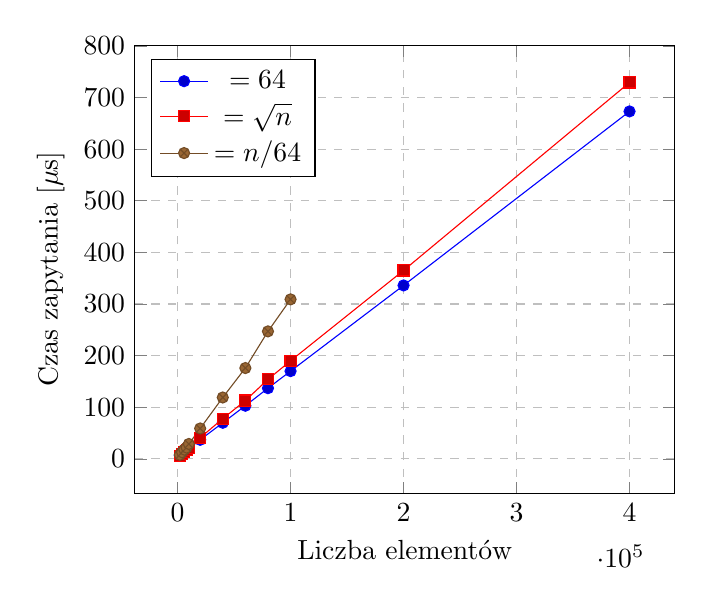
\begin{tikzpicture}
\begin{axis}[
    xlabel={Liczba elementów},
    ylabel={Czas zapytania [$\mu$s]},
    xmajorgrids=true,
    ymajorgrids=true,
    ytick={0, 100, 200, 300, 400, 500, 600, 700, 800},
    grid style=dashed,
    % xmode=log,
    % ymode=log,
    legend pos=north west,
]
\addplot coordinates{(2000, 6.623)(4000, 10)(6000, 13)(8000, 16)(10000, 20)(20000, 37)(40000, 70)(60000, 103)(80000, 137)(100000, 170)(200000, 336)(400000, 673)};
\addplot coordinates{(2000, 5.543)(4000, 10)(6000, 14)(8000, 18)(10000, 21)(20000, 41)(40000, 78)(60000, 113)(80000, 154)(100000, 190)(200000, 365)(400000, 729)};
\addplot coordinates{(2000, 7.918)(4000, 13)(6000, 18)(8000, 22)(10000, 29)(20000, 59)(40000, 119)(60000, 176)(80000, 247)(100000, 309)};
\legend{$\dt=64$,$\dt=\sqrt{n}$,$\dt={n/64}$}
\end{axis}
\end{tikzpicture}
\captionof{figure}{Czas zapytania algorytmu naiwnego}
\label{fig:plot-naive}
\end{minipage}
\hfill
\begin{minipage}[t]{0.49\textwidth}
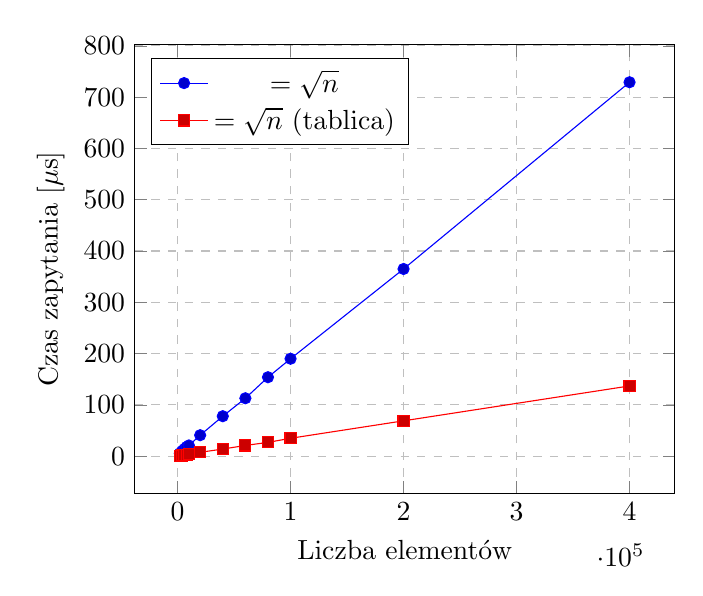
\begin{tikzpicture}
\begin{axis}[
    xlabel={Liczba elementów},
    ylabel={Czas zapytania [$\mu$s]},
    xmajorgrids=true,
    ymajorgrids=true,
    ytick={0, 100, 200, 300, 400, 500, 600, 700, 800, 900, 1000, 1180},
    grid style=dashed,
    % xmode=log,
    % ymode=log,
    legend pos=north west,
]
\addplot coordinates{(2000, 5.543)(4000, 10)(6000, 14)(8000, 18)(10000, 21)(20000, 41)(40000, 78)(60000, 113)(80000, 154)(100000, 190)(200000, 365)(400000, 729)};
\addplot coordinates{(2000, 0.751)(4000, 1.440)(6000, 2.115)(8000, 2.828)(10000, 3.561)(20000, 7.630)(40000, 14)(60000, 21)(80000, 27)(100000, 35)(200000, 69)(400000, 137)};
\legend{$\dt=\sqrt{n}$,$\dt=\sqrt{n}$ (tablica)}
\end{axis}
\end{tikzpicture}
\captionof{figure}{Porównanie dwóch wariantów}
\label{fig:plot-naive-variants}
\end{minipage}
W naszych danych oczekiwana długość zapytania zależy liniowo od liczby elementów, dlatego przewidujemy, że czas zapytania algorytmu naiwnego również będzie liniowy od rozmiaru. Dokładnie takie zachowanie obserwujemy na rysunku \ref{fig:plot-naive}. Ponadto możemy zauważyć, że algorytm naiwny dla liniowej liczby unikalnych elementów działa około półtora raza wolniej w porównaniu do innych kategorii danych. Podejrzewamy, że jest to spowodowane większą liczbą elementów w hash-mapie. Znalezienie odpowiedniej wartości może generować więcej nietrafień w pamięć podręczną procesora.

Tak jak podejrzewaliśmy, wariant drugi jest zdecydowanie szybszy (około 6 razy szybszy) w porównaniu do wariantu pierwszego. Operacje na hash-mapie, chociaż w teoretycznie czasie stałym, w praktyce są dużo wolniejsze od operacjach na tablicy.


\subsection{Algorytm offline}
\subsubsection{Czas inicjalizacji}
Czas inicjalizacji algorytmu offline w obu wariantach jest analogiczny do drugiego wariantu algorytmu naiwnego. W pierwszej implementacji przy użyciu binarnych drzew tworzymy tablicę zastępującą hash-mapę do zliczania elementów, a w przypadku drugim dodatkowo tworzymy tablicę list. W obu implementacjach czas inicjalizacji jest pomijalnie mały w porównaniu do czasu zapytania.
\subsubsection {Czas zapytania}
\begin{minipage}[t]{0.5\textwidth}
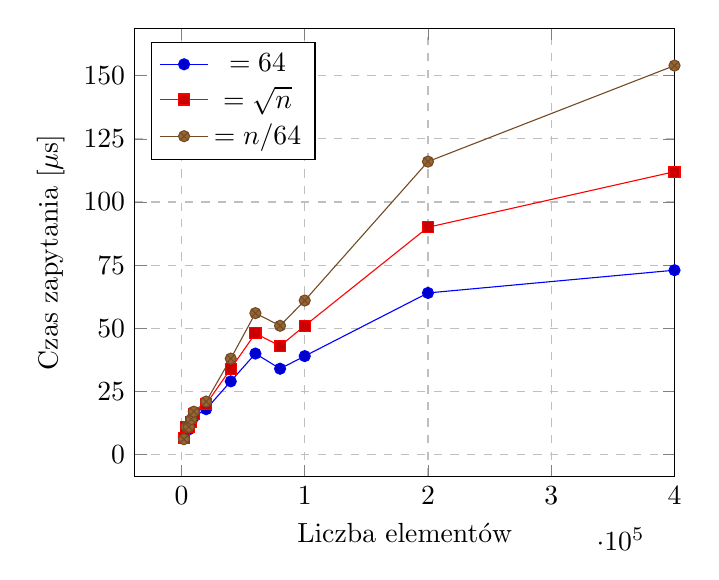
\begin{tikzpicture}
\begin{axis}[
    xlabel={Liczba elementów},
    ylabel={Czas zapytania [$\mu$s]},
    ytick={0, 25, 50, 75, 100, 125, 150},
    xmajorgrids=true,
    ymajorgrids=true,
    xmax=400000,
    grid style=dashed,
    legend pos=north west,
]
\addplot coordinates{(2000, 6.616)(4000, 11)(6000, 10)(8000, 13)(10000, 15)(20000, 18)(40000, 29)(60000, 40)(80000, 34)(100000, 39)(200000, 64)(400000, 73)};
\addplot coordinates{(2000, 6.459)(4000, 11)(6000, 11)(8000, 13)(10000, 16)(20000, 20)(40000, 34)(60000, 48)(80000, 43)(100000, 51)(200000, 90)(400000, 112)};
\addplot coordinates{(2000, 6.112)(4000, 11)(6000, 11)(8000, 14)(10000, 17)(20000, 21)(40000, 38)(60000, 56)(80000, 51)(100000, 61)(200000, 116)(400000, 154)};
\legend{$\dt=64$,$\dt=\sqrt{n}$,$\dt={n/64}$}
\end{axis}
\end{tikzpicture}
\captionof{figure}{Czas zapytania algorytmu offline BST}
\label{fig:plot-offline-bst}
\end{minipage}
\hfill
\begin{minipage}[t]{0.49\textwidth}
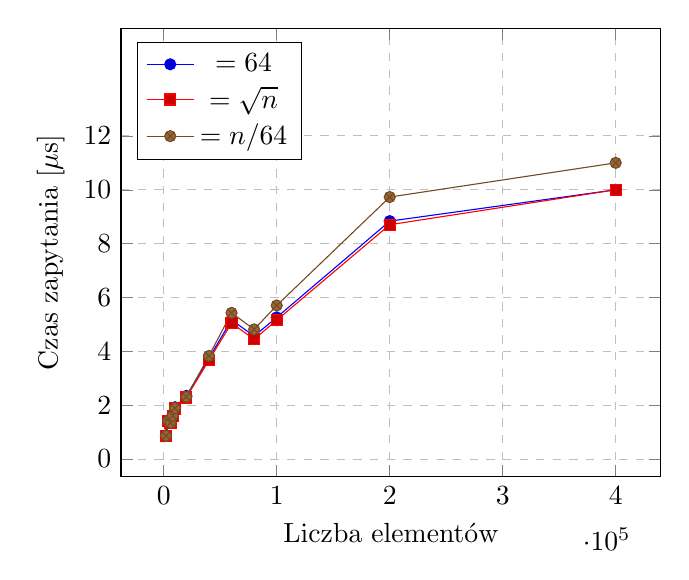
\begin{tikzpicture}
\begin{axis}[
    xlabel={Liczba elementów},
    ylabel={Czas zapytania [$\mu$s]},
    ymax=16,
    ytick={0, 2, 4, 6, 8, 10, 12},
    xmajorgrids=true,
    ymajorgrids=true,
    grid style=dashed,
    legend pos=north west,
]
\addplot coordinates{(2000, 0.881)(4000, 1.437)(6000, 1.356)(8000, 1.639)(10000, 1.923)(20000, 2.346)(40000, 3.744)(60000, 5.165)(80000, 4.569)(100000, 5.261)(200000, 8.836)(400000, 10)};
\addplot coordinates{(2000, 0.864)(4000, 1.404)(6000, 1.353)(8000, 1.603)(10000, 1.879)(20000, 2.286)(40000, 3.669)(60000, 5.049)(80000, 4.449)(100000, 5.158)(200000, 8.702)(400000, 10)};
\addplot coordinates{(2000, 0.865)(4000, 1.414)(6000, 1.343)(8000, 1.611)(10000, 1.892)(20000, 2.309)(40000, 3.830)(60000, 5.429)(80000, 4.816)(100000, 5.703)(200000, 9.730)(400000, 11)};
\legend{$\dt=64$,$\dt=\sqrt{n}$,$\dt={n/64}$}
\end{axis}
\end{tikzpicture}
\captionof{figure}{Czas zapytania algorytmu offline LIST}
\label{fig:plot-offline-list}
\end{minipage}
Dla danego rozmiaru tablicy wygenerowaliśmy liniową liczbę zapytań, dlatego przewidujemy czas działania $\Oh(\sqrt{n} \log n)$ w wersji \textsc{bst} oraz $\Oh(\sqrt{n})$ w wersji \textsc{list} dla pojedynczego zapytania. Zauważamy, że implementacja za pomocą tablicy list jest zdecydowanie lepsza, działa, aż $7$--$15$ razy szybciej. 
\subsubsection{Czas zapytania vs liczba zapytań}
\begin{minipage}[t]{0.5\textwidth}
\begin{tikzpicture}
\begin{axis}[
    xlabel={Liczba zapytań},
    ylabel={Łączny czas zapytań [s]},
    ytick={0, 10, 20, 30, 40, 50},
    xmajorgrids=true,
    ymajorgrids=true,
    grid style=dashed,
    legend pos=north west,
]
\addplot coordinates{(2000, 1.607)(4000, 2.002)(6000, 3.051)(8000, 3.242)(10000, 3.465)(20000, 5.923)(40000, 6.951)(60000, 7.867)(80000, 11)(100000, 12)(200000, 14)(400000, 25)};
\addplot coordinates{(2000, 1.436)(4000, 1.974)(6000, 3.211)(8000, 3.594)(10000, 3.911)(20000, 7.419)(40000, 9.342)(60000, 11)(80000, 17)(100000, 18)(200000, 22)(400000, 38)};
\addplot coordinates{(2000, 1.293)(4000, 1.982)(6000, 3.395)(8000, 3.929)(10000, 4.419)(20000, 8.618)(40000, 10)(60000, 12)(80000, 20)(100000, 21)(200000, 27)(400000, 52)};

\legend{$\dt=64$,$\dt=\sqrt{n}$,$\dt={n/64}$}
\end{axis}
\end{tikzpicture}
\captionof{figure}{Łączny czas zapytań algorytmu offline BST}
\label{fig:plot-offline-cum-bst}
\end{minipage}
\hfill
\begin{minipage}[t]{0.49\textwidth}
\begin{tikzpicture}
\begin{axis}[
    xlabel={Liczba zapytań},
    ylabel={Łączny czas zapytań [s]},
    ytick={0, 1, 2, 3, 4, 5},
    xmajorgrids=true,
    ymajorgrids=true,
    grid style=dashed,
    legend pos=north west,
]
\addplot coordinates{(2000, 0.238)(4000, 0.291)(6000, 0.450)(8000, 0.477)(10000, 0.504)(20000, 0.875)(40000, 1.010)(60000, 1.143)(80000, 1.760)(100000, 1.829)(200000, 2.172)(400000, 3.706)};
\addplot coordinates{(2000, 0.241)(4000, 0.295)(6000, 0.446)(8000, 0.472)(10000, 0.497)(20000, 0.854)(40000, 0.981)(60000, 1.104)(80000, 1.698)(100000, 1.773)(200000, 2.123)(400000, 3.638)};
\addplot coordinates{(2000, 0.229)(4000, 0.297)(6000, 0.445)(8000, 0.469)(10000, 0.492)(20000, 0.858)(40000, 0.998)(60000, 1.167)(80000, 1.794)(100000, 1.879)(200000, 2.295)(400000, 4.118)};
\legend{$\dt=64$,$\dt=\sqrt{n}$,$\dt={n/64}$}
\end{axis}
\end{tikzpicture}
\captionof{figure}{Łączny czas zapytań algorytmu offline LIST}
\label{fig:plot-offline-cum-list}
\end{minipage}
Algorytm offline jest jedynym opisanym przez nas algorytmem, którego czas działania zależy od liczby zapytań. Dlatego w trosce o kompletność przeprowadziliśmy testy sprawdzające jak zachowuje się algorytm offline w zależności od liczby zapytań. Zrobiliśmy testy dla $n=400000$.


\subsection{Struktury danych \textsc{CDLMW} oraz \textsc{CDLMW BP}}
\subsubsection{Czas inicjalizacji}
\begin{minipage}[t]{0.5\textwidth}
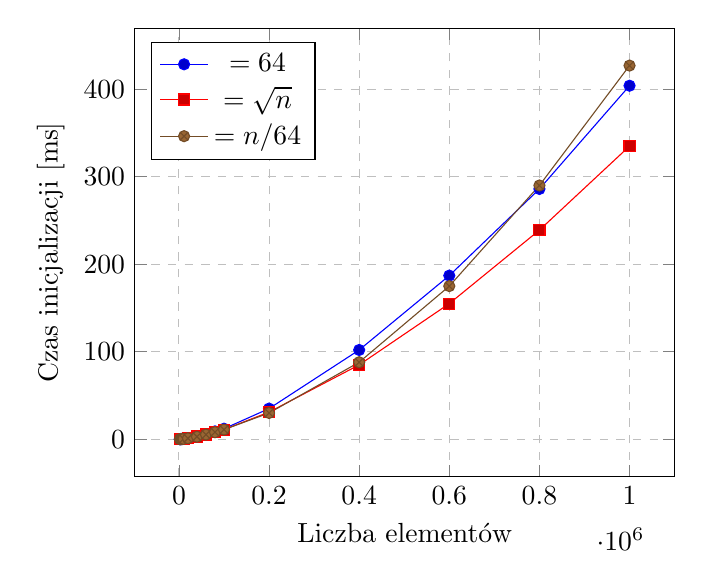
\begin{tikzpicture}
\begin{axis}[
    xlabel={Liczba elementów},
    ylabel={Czas inicjalizacji [ms]},
    ytick={0, 100, 200, 300, 400, 500},
    % ymin=80, ymax=50000,
    xmajorgrids=true,
    ymajorgrids=true,
    grid style=dashed,
    % xmode=log,
    % ymode=log,
    legend pos=north west,
]
\addplot coordinates{(2000, 0.047)(4000, 0.120)(6000, 0.211)(8000, 0.319)(10000, 0.494)(20000, 1.157)(40000, 3.190)(60000, 5.805)(80000, 8.947)(100000, 12)(200000, 35)(400000, 102)(600000, 187)(800000, 286)(1000000, 404)};
\addplot coordinates{(2000, 0.051)(4000, 0.121)(6000, 0.209)(8000, 0.314)(10000, 0.415)(20000, 1.116)(40000, 3.035)(60000, 5.412)(80000, 8.173)(100000, 11)(200000, 31)(400000, 85)(600000, 155)(800000, 239)(1000000, 335)};
\addplot coordinates{(2000, 0.055)(4000, 0.121)(6000, 0.206)(8000, 0.299)(10000, 0.399)(20000, 1.079)(40000, 2.892)(60000, 5.314)(80000, 8.051)(100000, 11)(200000, 30)(400000, 88)(600000, 175)(800000, 290)(1000000, 427)};
\legend{$\dt=64$,$\dt=\sqrt{n}$,$\dt={n/64}$}
\end{axis}
\end{tikzpicture}
\captionof{figure}{Czas inicjalizacji struktury danych \textsc{CDLMW}}
\label{fig:plot-init-cdlmw}
\end{minipage}
\hfill
\begin{minipage}[t]{0.49\textwidth}
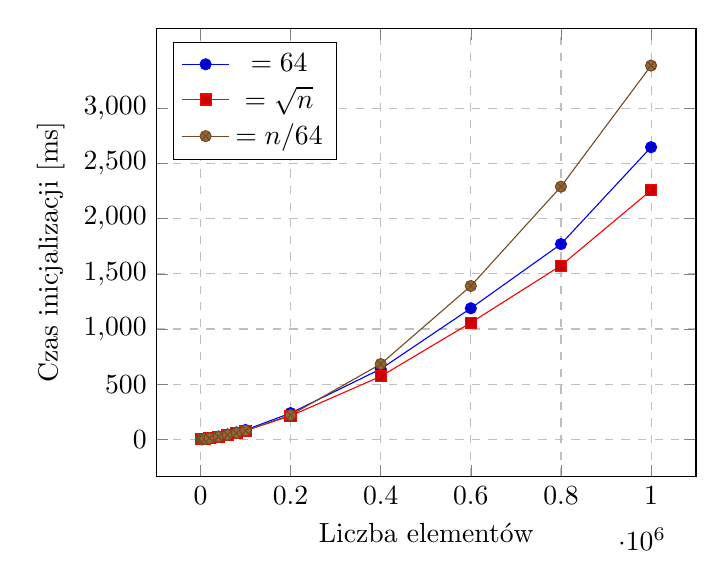
\begin{tikzpicture}
\begin{axis}[
    xlabel={Liczba elementów},
    ylabel={Czas inicjalizacji [ms]},
   ytick={0, 500, 1000, 1500, 2000, 2500, 3000},
    % ymin=80, ymax=50000,
    xmajorgrids=true,
    ymajorgrids=true,
    grid style=dashed,
    % xmode=log,
    % ymode=log,
    legend pos=north west,
]
\addplot coordinates{(2000, 0.607)(4000, 1.355)(6000, 2.213)(8000, 2.769)(10000, 3.963)(20000, 9.768)(40000, 24)(60000, 43)(80000, 61)(100000, 84)(200000, 237)(400000, 637)(600000, 1188)(800000, 1770)(1000000, 2649)};
\addplot coordinates{(2000, 0.621)(4000, 1.373)(6000, 2.208)(8000, 2.811)(10000, 3.946)(20000, 9.507)(40000, 23)(60000, 40)(80000, 57)(100000, 78)(200000, 212)(400000, 570)(600000, 1057)(800000, 1575)(1000000, 2258)};
\addplot coordinates{(2000, 0.639)(4000, 1.371)(6000, 2.191)(8000, 2.733)(10000, 3.902)(20000, 9.297)(40000, 23)(60000, 39)(80000, 56)(100000, 78)(200000, 219)(400000, 682)(600000, 1390)(800000, 2291)(1000000, 3389)};

\legend{$\dt=64$,$\dt=\sqrt{n}$,$\dt={n/64}$}
\end{axis}
\end{tikzpicture}
\captionof{figure}{Czas inicjalizacji struktury danych \textsc{CDLMW BP}}
\label{fig:plot-init-cdlmw-bp}
\end{minipage}

Przypominamy, że czas inicjalizacji struktur danych \textsc{CDLMW}, \textsc{CDLMW BP} wynosi odpowiednio $\Oh(n\sqrt{n})$, $\Oh(n\sqrt{nw})$. W naszej implementacji słowo maszynowe $w = 64$, więc bloki w wersji \textsc{BP} są $\sqrt{w}=8$ razy mniejsze. Z tego powodu spodziewamy się co najmniej $8$ razy wolniejszego czasu tworzenia struktury w wersji \textsc{BP}. W praktyce rozkłady $\dt=16$ oraz $\dt=\sqrt{n}$ radzą sobie lepiej, struktura \textsc{BP} działa około 6.5 razy wolniej. W przypadku dużej ilości unikalnych elementów struktura \textsc{BP} jest 8 razy wolniejsza.

Podejrzewaliśmy, że dodatkowa inicjalizacja \textsc{rank} oraz \textsc{select} w wersji \textsc{BP} struktury danych może mieć znaczący wpływ na czas konstrukcji. Po użyciu profilera\footnote{\url{https://perf.wiki.kernel.org/index.php/Tutorial}} dowiedzieliśmy się, że ponad $90\%$ czasu podczas inicjalizacji zajmuje obliczanie dominanty dla każdej pary bloków. Aby to potwierdzić postanowiliśmy zwiększyć liczbę bloków w algorytmie \textsc{CDLMW} do $\sqrt{nw}$. Otrzymaliśmy bardzo zbliżone czasy inicjalizacji do wersji \textsc{BP}.\vspace{-1.5em}
\subsubsection{Czas zapytania}
\begin{minipage}[t]{0.5\textwidth}
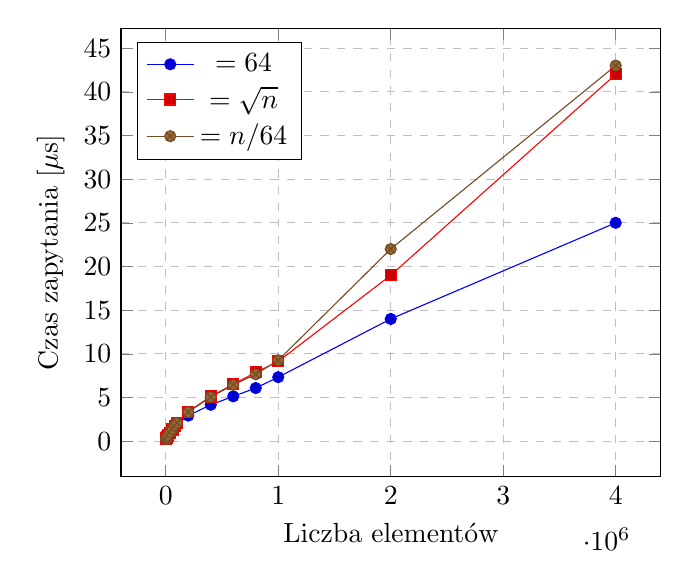
\begin{tikzpicture}
\begin{axis}[
    xlabel={Liczba elementów},
    ylabel={Czas zapytania [$\mu$s]},
    ytick={0, 5, 10, 15, 20, 25, 30, 35, 40, 45},
    xmajorgrids=true,
    ymajorgrids=true,
    grid style=dashed,
    legend pos=north west,
]
\addplot coordinates{(2000, 0.238)(4000, 0.317)(6000, 0.381)(8000, 0.431)(10000, 0.468)(20000, 0.645)(40000, 0.950)(60000, 1.318)(80000, 1.646)(100000, 1.948)(200000, 2.938)(400000, 4.174)(600000, 5.140)(800000, 6.089)(1000000, 7.338)(2000000, 14)(4000000, 25)};
\addplot coordinates{(2000, 0.237)(4000, 0.322)(6000, 0.385)(8000, 0.417)(10000, 0.474)(20000, 0.661)(40000, 0.977)(60000, 1.355)(80000, 1.711)(100000, 2.072)(200000, 3.392)(400000, 5.128)(600000, 6.523)(800000, 7.882)(1000000, 9.140)(2000000, 19)(4000000, 42)};
\addplot coordinates{(2000, 0.236)(4000, 0.318)(6000, 0.374)(8000, 0.430)(10000, 0.471)(20000, 0.678)(40000, 1.045)(60000, 1.392)(80000, 1.802)(100000, 2.091)(200000, 3.338)(400000, 5.064)(600000, 6.454)(800000, 7.669)(1000000, 9.270)(2000000, 22)(4000000, 43)};
\legend{$\dt=64$,$\dt=\sqrt{n}$,$\dt={n/64}$}
\end{axis}
\end{tikzpicture}
\captionof{figure}{Czas zapytania algorytmu \textsc{CDLMW}}
\label{fig:plot-cdlmw}
\end{minipage}
\hfill
\begin{minipage}[t]{0.49\textwidth}
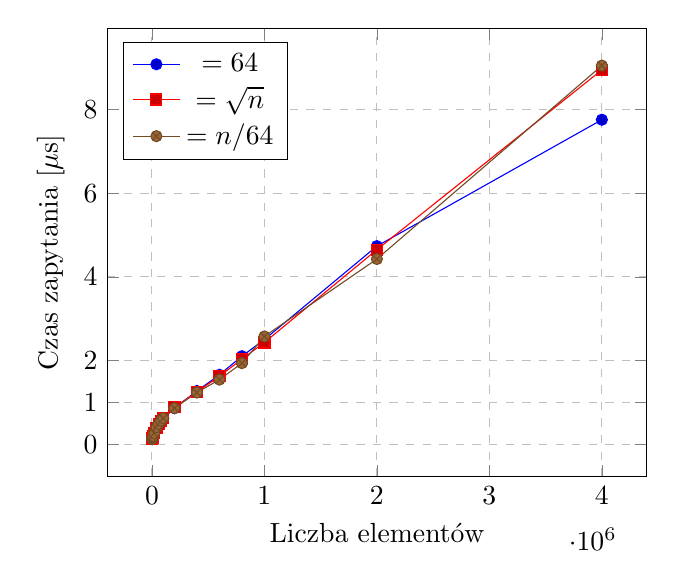
\begin{tikzpicture}
\begin{axis}[
    xlabel={Liczba elementów},
    ylabel={Czas zapytania [$\mu$s]},
    ytick={0, 1, 2, 4, 6, 8},
    xmajorgrids=true,
    ymajorgrids=true,
    grid style=dashed,
    legend pos=north west,
]
\addplot coordinates{(2000, 0.122)(4000, 0.139)(6000, 0.154)(8000, 0.176)(10000, 0.185)(20000, 0.252)(40000, 0.374)(60000, 0.470)(80000, 0.550)(100000, 0.619)(200000, 0.860)(400000, 1.270)(600000, 1.658)(800000, 2.102)(1000000, 2.501)(2000000, 4.733)(4000000, 7.753)};
\addplot coordinates{(2000, 0.122)(4000, 0.138)(6000, 0.154)(8000, 0.175)(10000, 0.185)(20000, 0.259)(40000, 0.381)(60000, 0.481)(80000, 0.557)(100000, 0.630)(200000, 0.885)(400000, 1.248)(600000, 1.625)(800000, 2.032)(1000000, 2.430)(2000000, 4.648)(4000000, 8.944)};
\addplot coordinates{(2000, 0.119)(4000, 0.138)(6000, 0.159)(8000, 0.173)(10000, 0.192)(20000, 0.261)(40000, 0.405)(60000, 0.482)(80000, 0.556)(100000, 0.621)(200000, 0.861)(400000, 1.235)(600000, 1.543)(800000, 1.937)(1000000, 2.575)(2000000, 4.425)(4000000, 9.047)};
\legend{$\dt=64$,$\dt=\sqrt{n}$,$\dt={n/64}$}
\end{axis}
\end{tikzpicture}
\captionof{figure}{Czas zapytania algorytmu \textsc{CDLMW BP}}
\label{fig:plot-cdlmw-bp}
\end{minipage}
Podczas zapytania w wersji \textsc{BP} skanujemy o jeden blok więcej, zatem oczekujemy, że zapytanie będzie $8 * (2/3)=5.33$ razy szybsze od wersji podstawowej algorytmu. W praktyce jednak tak nie jest, gdy liczba elementów jest mała doświadczamy około trzykrotnego przyśpieszenia. Wraz ze wzrostem liczby unikalnych elementów dostajemy około 4.75-krotne przyśpieszenie dla danych $\dt=\sqrt{n}$ oraz $\dt=n/64$.

\subsection{Struktura danych \textsc{CDLMW SF}}
\subsubsection{Czas inicjalizacji}
\begin{center}
    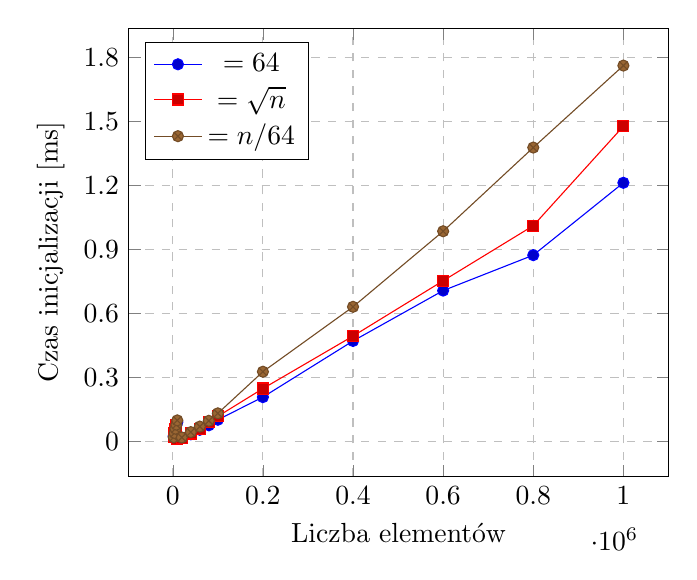
\begin{tikzpicture}
\begin{axis}[
    xlabel={Liczba elementów},
    ylabel={Czas inicjalizacji [ms]},
    ytick={0, 0.3, 0.6, 0.9, 1.2, 1.5, 1.8, 2.1},
    xmajorgrids=true,
    ymajorgrids=true,
    % ymax=12,
    grid style=dashed,
    legend pos=north west,
]
\addplot coordinates{(2000, 0.02573)(4000, 0.04133)(6000, 0.05831)(8000, 0.07721)(10000, 0.09082)(20000, 0.017)(40000, 0.034)(60000, 0.055)(80000, 0.076)(100000, 0.102)(200000, 0.208)(400000, 0.471)(600000, 0.707)(800000, 0.873)(1000000, 1.212)};
\addplot coordinates{(2000, 0.02295)(4000, 0.04040)(6000, 0.05831)(8000, 0.07662)(10000, 0.011)(20000, 0.017)(40000, 0.038)(60000, 0.059)(80000, 0.090)(100000, 0.118)(200000, 0.248)(400000, 0.494)(600000, 0.753)(800000, 1.011)(1000000, 1.477)};
\addplot coordinates{(2000, 0.02037)(4000, 0.03998)(6000, 0.06012)(8000, 0.07900)(10000, 0.09905)(20000, 0.019)(40000, 0.044)(60000, 0.070)(80000, 0.097)(100000, 0.132)(200000, 0.327)(400000, 0.631)(600000, 0.985)(800000, 1.377)(1000000, 1.761)};
\legend{$\dt=64$,$\dt=\sqrt{n}$,$\dt={n/64}$}
\end{axis}
\end{tikzpicture}
\captionof{figure}{Czas inicjalizacji struktury danych \textsc{CLDMW SF}}
\label{fig:plot-init-cdlmw-sf}
\end{center}
Czas inicjalizacji struktury danych \textsc{CDLMW SF} zależy liniowo od rozmiaru tablicy. Na wykresie \ref{fig:plot-init-cdlmw-sf} możemy zaobserwować, że w praktyce im więcej unikalnych elementów tym większy czas inicjalizacji.
\subsubsection{Czas zapytania}
\begin{minipage}[t]{0.5\textwidth}
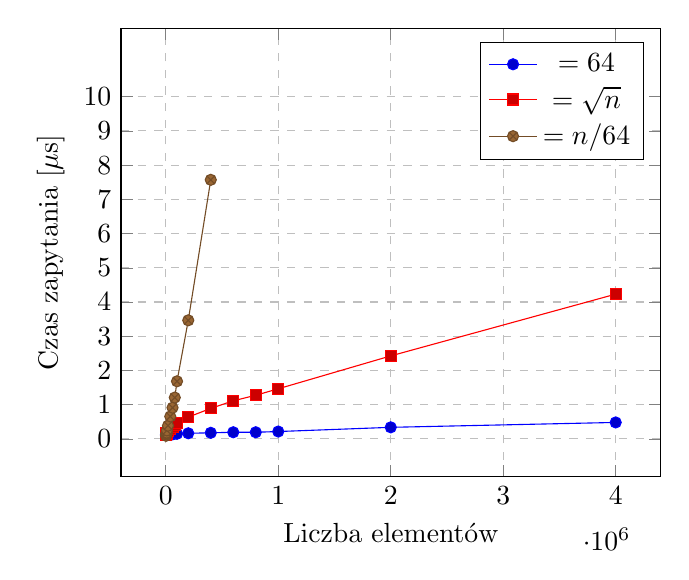
\begin{tikzpicture}
\begin{axis}[
    xlabel={Liczba elementów},
    ylabel={Czas zapytania [$\mu$s]},
    ytick={0, 1, 2, 3, 4, 5, 6, 7, 8, 9, 10},
    xmajorgrids=true,
    ymajorgrids=true,
    ymax=12,
    grid style=dashed,
    legend pos=north east,
]
\addplot coordinates{(2000, 0.125)(4000, 0.128)(6000, 0.133)(8000, 0.125)(10000, 0.130)(20000, 0.138)(40000, 0.128)(60000, 0.133)(80000, 0.155)(100000, 0.150)(200000, 0.164)(400000, 0.178)(600000, 0.194)(800000, 0.194)(1000000, 0.215)(2000000, 0.338)(4000000, 0.481)};
\addplot coordinates{(2000, 0.106)(4000, 0.130)(6000, 0.160)(8000, 0.154)(10000, 0.173)(20000, 0.242)(40000, 0.299)(60000, 0.350)(80000, 0.417)(100000, 0.468)(200000, 0.636)(400000, 0.892)(600000, 1.113)(800000, 1.275)(1000000, 1.464)(2000000, 2.425)(4000000, 4.230)};
\addplot coordinates{(2000, 0.091)(4000, 0.129)(6000, 0.161)(8000, 0.183)(10000, 0.247)(20000, 0.386)(40000, 0.656)(60000, 0.911)(80000, 1.208)(100000, 1.683)(200000, 3.465)(400000, 7.570)};
\legend{$\dt=64$,$\dt=\sqrt{n}$,$\dt={n/64}$}
\end{axis}
\end{tikzpicture}
\captionof{figure}{Czas zapytania algorytmu \textsc{CLDMW SF} z optymalizacjami}
\label{fig:plot-cdlmw-sf}
\end{minipage}
\hfill
\begin{minipage}[t]{0.49\textwidth}
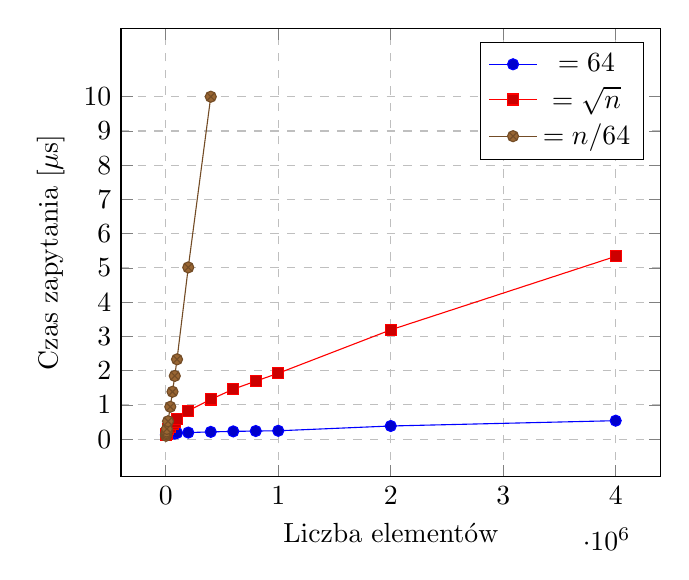
\begin{tikzpicture}
\begin{axis}[
    xlabel={Liczba elementów},
    ylabel={Czas zapytania [$\mu$s]},
    ytick={0, 1, 2, 3, 4, 5, 6, 7, 8, 9, 10},
    ymax=12,
    xmajorgrids=true,
    ymajorgrids=true,
    grid style=dashed,
    legend pos=north east,
]
\addplot coordinates{(2000, 0.135)(4000, 0.142)(6000, 0.151)(8000, 0.147)(10000, 0.145)(20000, 0.144)(40000, 0.149)(60000, 0.165)(80000, 0.163)(100000, 0.182)(200000, 0.193)(400000, 0.213)(600000, 0.227)(800000, 0.238)(1000000, 0.245)(2000000, 0.385)(4000000, 0.540)};
\addplot coordinates{(2000, 0.116)(4000, 0.144)(6000, 0.162)(8000, 0.180)(10000, 0.190)(20000, 0.291)(40000, 0.366)(60000, 0.441)(80000, 0.505)(100000, 0.578)(200000, 0.834)(400000, 1.161)(600000, 1.460)(800000, 1.695)(1000000, 1.925)(2000000, 3.192)(4000000, 5.339)};
\addplot coordinates{(2000, 0.099)(4000, 0.145)(6000, 0.182)(8000, 0.225)(10000, 0.300)(20000, 0.523)(40000, 0.946)(60000, 1.385)(80000, 1.847)(100000, 2.331)(200000, 5.016)(400000, 10)};

\legend{$\dt=64$,$\dt=\sqrt{n}$,$\dt={n/64}$}
\end{axis}
\end{tikzpicture}
\captionof{figure}{Czas zapytania algorytmu \textsc{CDLMW SF} bez optymalizacji}
\label{fig:plot-cdlmw-sf-noop}
\end{minipage}
Testy czasu zapytań przeprowadziliśmy dla dwóch wersji struktury \textsc{CDLMW SF}: z optymalizacjami opisanych w sekcji \ref{sec:cdlmw-sf-impl}, oraz bez optymalizacji. Wyniki testów można zobaczyć odpowiednio na rysunkach \ref{fig:plot-cdlmw-sf} oraz \ref{fig:plot-cdlmw-sf-noop}. Dla danych z stałą liczbą unikalnych elementów czas zapytania w obu wersjach jest praktycznie taki sam. Dla kategorii $\dt=\sqrt{n}$ oraz $\dt=n/64$ zoptymalizowana wersja jest o około 1.25 razy szybsza od podstawowej.
\subsection{Struktura danych \textsc{CDLMW BP + SF}}
\begin{minipage}[t]{0.5\textwidth}
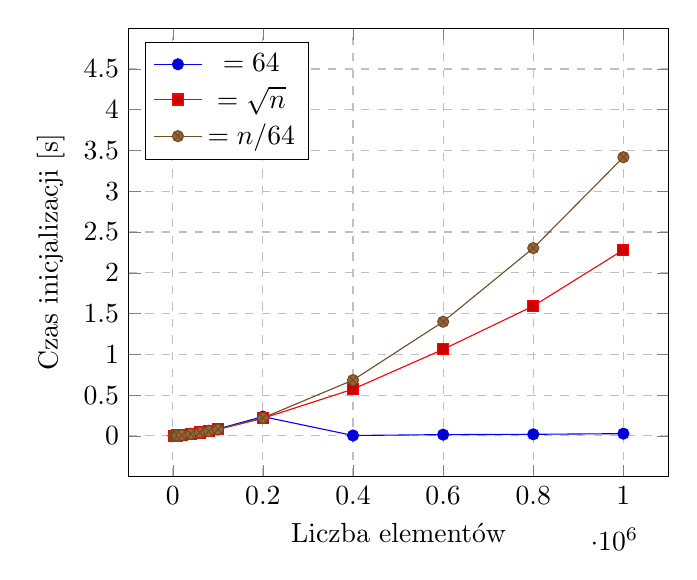
\begin{tikzpicture}
\begin{axis}[
    xlabel={Liczba elementów},
    ylabel={Czas inicjalizacji [s]},
    log ticks with fixed point,
    xmajorgrids=true,
    ymajorgrids=true,
    ytick={0,0.5,1,1.5,2,2.5,3,3.5,4,4.5},
    ymax=5,
    grid style=dashed,
    legend pos=north west,
]
\addplot coordinates{(2000, 0.000627)(4000, 0.001395)(6000, 0.002287)(8000, 0.002921)(10000, 0.004082)(20000, 0.010)(40000, 0.025)(60000, 0.043)(80000, 0.062)(100000, 0.085)(200000, 0.236)(400000, 0.004438)(600000, 0.015)(800000, 0.019)(1000000, 0.027)};
\addplot coordinates{(2000, 0.000632)(4000, 0.001400)(6000, 0.002244)(8000, 0.002855)(10000, 0.004069)(20000, 0.009641)(40000, 0.023)(60000, 0.041)(80000, 0.058)(100000, 0.079)(200000, 0.215)(400000, 0.573)(600000, 1.061)(800000, 1.592)(1000000, 2.281)};
\addplot coordinates{(2000, 0.000641)(4000, 0.001399)(6000, 0.002230)(8000, 0.002781)(10000, 0.003944)(20000, 0.009439)(40000, 0.023)(60000, 0.040)(80000, 0.057)(100000, 0.079)(200000, 0.220)(400000, 0.684)(600000, 1.400)(800000, 2.303)(1000000, 3.418)};
\legend{$\dt=64$,$\dt=\sqrt{n}$,$\dt={n/64}$}
\end{axis}
\end{tikzpicture}
\captionof{figure}{Czas inicjalizacji struktury danych \textsc{CLDMW BP + SF}}
\label{fig:plot-init-cdlmw-bp-sf}
\end{minipage}
\hfill
\begin{minipage}[t]{0.49\textwidth}
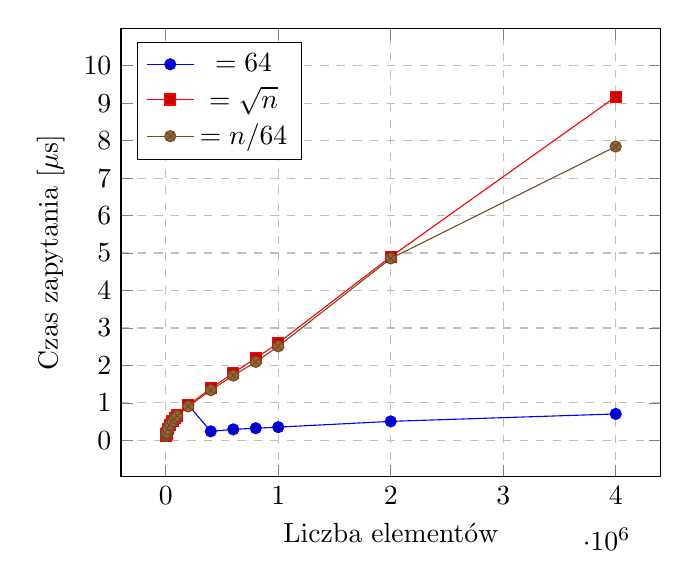
\begin{tikzpicture}
\begin{axis}[
    xlabel={Liczba elementów},
    ylabel={Czas zapytania [$\mu$s]},
    log ticks with fixed point,
    xmajorgrids=true,
    ymajorgrids=true,
    ytick={0,1,2,3,4,5,6,7,8,9,10},
    ymax=11,
    grid style=dashed,
    legend pos=north west,
]
\addplot coordinates{(2000, 0.125)(4000, 0.146)(6000, 0.165)(8000, 0.187)(10000, 0.204)(20000, 0.291)(40000, 0.413)(60000, 0.503)(80000, 0.596)(100000, 0.663)(200000, 0.941)(400000, 0.240)(600000, 0.293)(800000, 0.324)(1000000, 0.353)(2000000, 0.507)(4000000, 0.705)};
\addplot coordinates{(2000, 0.128)(4000, 0.146)(6000, 0.166)(8000, 0.188)(10000, 0.204)(20000, 0.296)(40000, 0.414)(60000, 0.509)(80000, 0.605)(100000, 0.663)(200000, 0.940)(400000, 1.387)(600000, 1.797)(800000, 2.193)(1000000, 2.600)(2000000, 4.901)(4000000, 9.170)};
\addplot coordinates{(2000, 0.122)(4000, 0.144)(6000, 0.168)(8000, 0.188)(10000, 0.205)(20000, 0.300)(40000, 0.418)(60000, 0.505)(80000, 0.596)(100000, 0.654)(200000, 0.906)(400000, 1.339)(600000, 1.728)(800000, 2.094)(1000000, 2.509)(2000000, 4.855)(4000000, 7.842)};
\legend{$\dt=64$,$\dt=\sqrt{n}$,$\dt={n/64}$}
\end{axis}
\end{tikzpicture}
\captionof{figure}{Czas zapytania struktury danych \textsc{CLDMW BP + SF}}
\end{minipage}
\paragraph{Czas inicjalizacji} Przypominamy, że czas inicjalizacji struktury \textsc{CDLMW BP + SF} wynosi $\Oh(n\sqrt{nw})$. Dla kategorii danych $\dt=64$ oraz $\dt=\sqrt{n}$ wykres \ref{fig:plot-init-cdlmw-bp-sf} to odzwierciedla, aczkolwiek dla typu $\dt=64$ przy $n=4*10^4$ elementów następuje nagły spadek czasu inicjalizacji. Wynika to z faktu, że dla kategorii $\dt=64$ oraz $n \ge 512^2 \approx 2.6*10^5$ oczekiwana częstotliwość każdego elementu jest większa niż $\sqrt{nw}$, przez co wszystkie elementy są obsługiwane przez podstrukturę \textsc{CDLMW SF}, która to ma znacznie szybszy, liniowy, czas inicjalizacji.

\subsection{Podsumowanie}
W sekcji tej postaramy się odpowiedzieć na pytanie jakiego algorytmu/struktury danych należy użyć, aby rozwiązać problem \textsc{RMQ} jak najszybciej.

\paragraph{Algorytm naiwny} Polecamy użyć algorytmu naiwnego w przypadku, gdy suma długości przedziałów zapytań nie przekracza $n$. Wszystkie opisane struktury danych potrzebują co najmniej linowego czasu na inicjalizację, czas ten równie dobrze możemy zagospodarować na obliczanie dominanty.

\paragraph{Algorytm offline} Na wstępie zauważamy, że nie ma sensu używać wariantu \textsc{BST}, jest on od 7 do 15 razy wolniejszy od wersji \textsc{LIST}. Gdy algorytm $\alpha$ rozwiązujący problem \textsc{RMQ} działa w czasie $f(n) \ge \log n$ to używamy algorytmu offline\footnote{O ile wszystkie zapytania są dostępne a priori}, gdy liczba zapytań $|Q| \ge C (n/f(x))^2$ dla odpowiednio dobranej stałej $C$\footnote{Wszystkie stałe w tym podrozdziale zostały dobrane przez dodatkowe eksperymenty}. Dla takiego doboru $|Q|$ algorytm offline działa nie wolniej niż algorytm $\alpha$. W szczególności dla algorytmów \textsc{CDLMW SF} oraz \textsc{CDLMW BP + SF} dobieramy liczbę zapytań odpowiednio $128(n/\dt)^2$ oraz $2(n/\sqrt{n/w})^2$ dla których algorytm offline \textsc{LIST} osiąga podobne czasy zapytań.

\paragraph{Struktura danych \textsc{KMS}} Nie zalecamy używać tej struktury, struktura \textsc{CDLMW} posiada praktycznie identyczny czas inicjalizacji i jednocześnie szybszą operacje \textsc{query}.

\paragraph{Struktura danych \textsc{CDLMW SF}} Gdy unikalnych elementów nie jest więcej niż $45\sqrt{n/w}$ proponujemy użyć struktury \textsc{CDLMW SF}, posiada ona liniowy czas inicjalizacji oraz czas zapytania jest najszybszy ze wszystkich struktury danych przy tej dystrybucji danych.

\paragraph{Struktury danych \textsc{CDLMW BP + SF}}
Gdy unikalnych elementów jest więcej niż $45\sqrt{n/w}$ sugerujemy użycie struktury \textsc{CDLMW BP + SF}. Niestety czas inicjalizacji jest znacząco gorszy w porównaniu do struktury \textsc{CDLMW SF}, aczkolwiek czas zapytania jest co najmniej dwukrotnie szybszy.
% \paragraph{Pierwszy przypadek $\dt \le \sqrt{n}$}